\documentclass[paper=letter,fontsize=11pt,captions=tableheading]{scrartcl}
\usepackage[american]{babel}
\usepackage[latin1]{inputenc}
\usepackage[T1]{fontenc}
%\usepackage[top=1in,bottom=1in,left=1in,right=1in]{geometry}
\usepackage{lmodern}

\usepackage{amsmath}
\usepackage{amssymb}

\usepackage[amsmath,hyperref,thmmarks]{ntheorem}
\usepackage{graphicx}
\usepackage[
	bookmarks,
	colorlinks=false,
	linkcolor=blue,
	citecolor=blue,
	pagebackref=false,
	pdftitle={CloudKeeper Design Document},
	pdfauthor={SVBio},
	pdfsubject={},
	pdfkeywords={}
]{hyperref}
\usepackage{scrpage2}                  % Headers and footers
\usepackage{color}                     % Colors, possibly only for \todo
\usepackage{enumitem}                  % enumerate environment
\usepackage{subcaption}
\usepackage{xspace}                    % Correct spaces after \newcommand definitions
\usepackage[noend]{algpseudocode}      % algorithm environment

% BEGIN Doc Layout
	\allowdisplaybreaks[3]

	\setkomafont{disposition}{\normalcolor\bfseries}
	\setkomafont{descriptionlabel}{\bfseries}
	\setkomafont{captionlabel}{\usekomafont{disposition}}

	\setlength{\arrayrulewidth}{.5pt}
	\numberwithin{equation}{section}
	\renewcommand{\theenumi}{\roman{enumi}}
	\renewcommand{\labelenumi}{\theenumi)}

	\newcommand{\otoprule}{\midrule[\heavyrulewidth]}

	\setcounter{secnumdepth}{3}

	\makeatletter
	% Algorithms are expected to have an optional argument of form
	% FunctionName$(ArgumentList)$, e.g., DiscreteSample$(A, w)$
	\def\internal@funcName#1$(#2)${#1}
	\newcommand\funcName[1]{\internal@funcName #1}
	\newtheoremstyle{algorithm}
		{\item[\rlap{\vbox{\hbox{\hskip\labelsep \theorem@headerfont
			##1\ ##2\theorem@separator}\hbox{\strut}}}]}%
		{\item[\rlap{\vbox{\hbox{\hskip\labelsep {\theorem@headerfont
			##1}\ \normalfont\texttt{##3}{\theorem@headerfont\theorem@separator}}\hbox{\strut}}}]%
			\def\@currentlabel{\texttt{\funcName{##3}}}}
	\makeatother
% END Doc Layout

% BEGIN General Definitions
	\newcommand{\todo}[1]{\textbf{\color{red}#1}}

	\newcommand{\specialcell}[3][t]{%
		\begin{tabular}[#1]{@{}#2@{}}#3\end{tabular}}

	% BEGIN Mathematical Definition
		% Space (only) in displaymath (e.g., between mathematical expression and punctuation mark)
		\newcommand{\SiM}{\mathchoice{\,}{}{}{}}
	% END Mathematical Operators

	% BEGIN URLs
		\newcommand{\mailto}[1]{\href{mailto:#1}{\nolinkurl{#1}}}
		\newcommand{\doi}[1]{DOI: \href{http://dx.doi.org/#1}{\nolinkurl{#1}}}
	% END URLs

	\makeatletter
	% BEGIN Mathematical Definitions
		% BEGIN Set Symbols
			\newcommand{\setsymbol}[1]{\mathbb{#1}}
			\newcommand{\N}{\@ifstar{\setsymbol{N}_0}{\setsymbol{N}}}
			\newcommand{\R}{\setsymbol{R}}
		    \newcommand{\Nupto}{\@ifstar{\Nupto@star}{\Nupto@nostar}}
		    \newcommand{\Nupto@star}[1]{[#1]_0}
		    \newcommand{\Nupto@nostar}[1]{[#1]}
		% END Set Symbols
		\renewcommand{\vec}[1]{\ensuremath{\boldsymbol{#1}}}
		\newcommand{\pow}[1]{2^{#1}}
	% END Mathematical Definitions
	\makeatother

	\renewcommand{\vec}[1]{\ensuremath{\boldsymbol{#1}}}
	\newcommand{\enumref}[1]{(\ref{#1})}

	\makeatletter
	\newcommand{\symlabel}[2]{\def\@currentlabel{\texttt{#1}}\texttt{#1}\label{#2}}
	\makeatother

	\newcommand{\Warning}[1]{\marginpar[\HandRight]{\HandLeft}\textbf{#1}}

	% BEGIN Algorithms
	\theoremstyle{algorithm}
	\theorembodyfont{\upshape}
	\newtheorem{algorithm}{Algorithm}[section]

	\newlength{\alglabelwidth}
	\newcommand{\alginput}[1]{%
		\par\noindent%
		\settowidth{\alglabelwidth}{\emph{Require:}}%
		\makebox[\alglabelwidth][l]{\emph{Input:}} \begin{tabular}[t]{l} #1 \end{tabular}}
	\newcommand{\algoutput}[1]{%
		\par\noindent%
		\settowidth{\alglabelwidth}{\emph{Require:}}%
		\makebox[\alglabelwidth][l]{\emph{Output:}} \begin{tabular}[t]{l} #1 \end{tabular}}
	\newcommand{\algprecond}[1]{%
		\par\noindent%
		\settowidth{\alglabelwidth}{\emph{Require:}}%
		\makebox[\alglabelwidth][l]{\emph{Require:}} \begin{tabular}[t]{l} #1 \end{tabular}}
	\algnewcommand{\LineComment}[1]{\State $\triangleright$ #1}

	\newcommand{\set}{\leftarrow}
	\DeclareMathOperator{\random}{random}
	\newcommand{\dist}{\ensuremath{\mathit{dist}}}
	\newcommand{\List}{\mathrm{List}}
	\newcommand{\Sample}{\mathit{Sample}}
	\algblockdefx[With]{With}{EndWith}%
		[1]{\textbf{with} #1 \textbf{do}}%
		[0]{End}
	\algnotext[With]{EndWith}
	% END Algorithms

	% BEGIN Theorem environments
		\theoremstyle{plain}
		\theoremseparator{.}

		\theoremheaderfont{\itshape}
		\newtheorem{claim}[equation]{Claim}

		\theoremheaderfont{\normalfont\bfseries}
		\theorembodyfont{\itshape}
		\newtheorem{theorem}[equation]{Theorem}
		\newtheorem{lemma}[equation]{Lemma}
		\newtheorem{corollary}[equation]{Corollary}

		\theorembodyfont{\normalfont}
		\theoremsymbol{$\lozenge$}
		\newtheorem{definition}[equation]{Definition}
		\newtheorem{example}[equation]{Example}

		\theoremstyle{nonumberplain}
		\theoremheaderfont{\itshape}
		\theoremsymbol{$\square$}
		\newtheorem{proof}{Proof}

		\theoremsymbol{$\blacksquare$}
		\newtheorem{subproof}{Proof}
	% END Theorem environments
% END General Definitions

\graphicspath{{figures/}}

\title{CloudKeeper}

\author{Florian Schoppmann\thanks{\mailto{fschoppmann@lifecodehealth.com}}}

\begin{document}

\maketitle

\begin{abstract}
This article introduces CloudKeeper: a domain-specific language and a corresponding runtime system for data flows. While motivated by Lifecode's needs of analyzing the human genome at scale, CloudKeeper is entirely general-purpose and abstracts away tasks like data transfer, serialization, scheduling, checkpointing, and package/dependency management. For Lifecode this means, e.g., that without any source-code modifications, our genome-analysis data flow can be run purely in-memory within a single JVM as well as in a distributed fashion in the cloud.

CloudKeeper is superficially similar to academic workflow management systems like Taverna or Pegasus, though it targets software engineers instead of users. The statically typed DSL piggybacks on existing IDE support for Java, Scala, or Groovy -- it also allows seamless integration of data-flow programming into any JVM-based language. The runtime system is available as just a library, and it is lightweight enough to be used as alternative to lower-level parallelization concepts such as threads, Java executor services, actor systems, futures/promises etc. CloudKeeper is highly modular and versatile: E.g., intermediate results can be kept as in-memory Java objects as well as in the file system or in a cloud-storage service. Likewise, processing of individual tasks can be as different as using an existing thread pool or by submitting a job to a distributed resource manager like Grid Engine.

Besides explaining CloudKeeper's design philosophy and architecture, this article also introduces the sophisticated data-flow-execution and checkpointing algorithms use by CloudKeeper, including formal correctness proofs.
\end{abstract}

\section{Introduction}

\todo{Write an introduction and present related work!}

\section{The Interpreter Component} \label{ch:interpreter}

The \emph{CloudKeeper interpreter} component is responsible for traversing the runtime representation of a workflow (in the terminology of programming languages and compilers, this is sometimes referred to as the \emph{optimized abstract-syntax tree}) and for recursively starting interpreters for submodules. It provides different kinds of module interpreters corresponding to the different kinds of CloudKeeper modules, such as composite modules, loop modules, or simple modules.

Most of the complexity of the interpreter component stems from parent modules. Simple modules instead are atomic entities for the interpreter, as they consist of user-defined code written in Java or some other programming language. Therefore, a simple-module interpreter simply passes the simple module on to the \emph{executor} component, which is responsible for executing user-defined code. An executor has a great degree of freedom in doing so: For instance, it may invoke the user-defined code on a remote machine, make use of external schedulers, etc. However, the details of executors are entirely hidden from a simple-module interpreter and therefore do not need to be addressed in this section.

\subsection{Formal Model of CloudKeeper Modules}

\newcommand{\children}[1]{\operatorname{ch}(#1)}
\newcommand{\ports}[1]{\operatorname{ports}(#1)}
\newcommand{\conn}[1]{\operatorname{conn}(#1)}
\newcommand{\dir}[1]{\operatorname{dir}(#1)}
\newcommand{\incoming}{\text{in}}
\newcommand{\outgoing}{\text{out}}
\newcommand{\fromport}[1]{\operatorname{from}(#1)}
\newcommand{\toport}[1]{\operatorname{to}(#1)}
\newcommand{\module}[1]{\operatorname{module}(#1)}
\newcommand{\deps}{\operatorname{deps}}
\newcommand{\val}{\ensuremath{\bullet}} % has value
\newcommand{\optv}{\ensuremath{\circ}} % has optional value
\newcommand{\nval}{\ensuremath{\cdot}} % no value
\newcommand{\pred}{\operatorname{pred}}
\newcommand{\suc}{\operatorname{suc}}
\newcommand{\state}{\mathit{state}}
\newcommand{\irrelevant}{\mathit{irrelevant}}
\newcommand{\ready}{\mathit{ready}}
\newcommand{\recompute}{\mathit{recompute}}
\newcommand{\outports}{\operatorname{outports}}
\newcommand{\Cparentchild}{C_{\uparrow}}
\newcommand{\Csibling}{C^{\to}}
\newcommand{\Cchildparent}{C^{\downarrow}}
\newcommand{\Cshort}{C_{\to}}

In order to reason about the concepts used by the CloudKeeper interpreter component as well as to prove correctness of the algorithms described in this section, we start by introducing a formal model of what constitutes CloudKeeper modules. This is followed by additional definitions needed later, as well as a concrete example.

\paragraph{Modules}

A \emph{CloudKeeper module} is a 6-tuple $M = (I, O, L, \deps, S, C)$ consisting of the following elements.
%
\begin{itemize}
	\item A set $I$ of in-ports. An in-port is a formal input parameter.
	\item A set $O$ of out-ports. An out-port is a formal output parameter.
	\item A set $L$ of in-port/out-port pairs each of which defines an I/O-port. If $M$ is not a loop module, then necessarily $L = \emptyset$.
	\item A function $\deps: I \to \pow O$ that maps each in-port $i \in I$ to a subset of out-ports. If $o \in \deps(i)$ we say that out-port $o$ \emph{depends} on in-port $i$. While it is necessary that $o \in \deps(i)$ if the value passed for $i$ is needed for computing the value of $o$, there is no upper-bound constraint on $\deps(i)$. In other words, $\deps(i) = O$ is always valid.
	\item A set $S$ of submodules, where every $N \in S$ is itself a module $N = (I_N, O_N, L_N, \deps_N, S_N, C_N)$. If $M$ is not a parent module, then necessarily $S = \emptyset$.
	\item A set $C$ of connections. Each connection $c \in C$ is an ordered pair of ports in the union of $I$, $O$, and all in\nobreakdash- and out-ports of (direct) submodules of $M$. When $M$ is not a parent module, then necessarily $C = \emptyset$.

	The set $C$ can be partitioned into the set of \emph{parent-in-to-child-in} connections $\Cparentchild$, the set of \emph{sibling connections} $\Csibling$, the set of \emph{child-out-to-parent-out} connections $\Cchildparent$, and the set of \emph{short-circuit} connections $\Cshort$. Specifically, let $c = (p,q) \in C$. Then:
		\begin{enumerate}
			\item $c \in \Cparentchild$ if $p \in I$ and $\exists N \in S: q \in I_N$
			\item $c \in \Cchildparent$ if $\exists N \in S: p \in O_N$ and $q \in O$
			\item $c \in \Csibling$ if $\exists N, P \in S: p \in O_N$ and $q \in I_P$
			\item $c \in \Cshort$ if $p \in I$ and $q \in O$
		\end{enumerate}
\end{itemize}

\paragraph{Graphs}

A \emph{directed graph} $G = (V, E)$ consists of a set of \emph{vertices} $V$ and a set of \emph{edges} $E \subseteq V^2$. A vertex $v \in V$ is called a \emph{source vertex} is it has no incoming edges, that is, there is no $w \in V$ with $(w,v) \in E$. Likewise, $v$ is called a \emph{sink vertex} if it has no outgoing edges, that is, there is no $w \in V$ with $(v,w) \in E$. A \emph{path} of length $n \geq 0$ is a sequence of vertices $(v_0, \dots, v_n)$ so that for every $i = 1, \dots, n$, it holds that $(v_{i-1}, v_i) \in E$. The path is called \emph{maximal} if $v_0$ is a source vertex and $v_n$ is a sink vertex.

Given a vertex $v \in V$, we say that another $w \in V$ is \emph{reachable from $v$} if there is a path from $v$ to $w$. Corresponding to the previous definition of a path, the reachable relation is reflexive; that is, every vertex is reachable from itself.


\paragraph{Dependency Graphs}

Let $M = (I, O, L, \deps, S, C)$ be a module. Define $V :=  S \cup I \cup O \cup \left( \bigcup_{N \in S} I_N \right)$ as the set of all submodules, all in-port, all out-ports, and all submodules' in-ports. The \emph{dependency graph of $M$} is then defined as the directed graph $G = (V,E)$, where the edge set~$E$ contains $(v,w)$ if and only if one of the following (mutually exclusive) conditions holds:
\begin{enumerate}
	\item $(v,w)$ is a parent-in-to-child-in or a short-circuit connection. Formally, $(v,w) \in \Cparentchild \cup \Cshort$.
	\item \label{def:depgraph:E:cond2} $v$ is the in-port of some submodule, and this submodule has an out-port that depends on $v$ and that has a connection to $w$. Formally, $\exists N \in S: v \in I_N$ and $\exists o \in \deps_N(v): (o,w) \in \Csibling \cup \Cchildparent$.
	\item \label{def:depgraph:E:cond3} $v$ is a submodule, $w$ is an out-port or a submodule's in-port, and $v$ has an out-port that has a connection to $w$. Formally, $\exists N \in S: v = N$ and $\exists o \in O_N: (o,w) \in \Csibling \cup \Cchildparent$.
\end{enumerate}

Let $R := \bigcup_{N \in S} O_N$ be the set of all submodules' out-ports. We define $\outports(v,w): E \to \pow R$ as the set of all out-ports that \emph{witness} the connection between $v$ and $w$ in the dependency graph (in case of conditions~\eqref{def:depgraph:E:cond2} and \eqref{def:depgraph:E:cond3}). Formally,
\begin{equation*}
	\outports(v,w) := \begin{cases}
		\emptyset & \text{if $v \in I$} \\
		\{ o \in \deps_N(v) \mid (o,w) \in \Csibling \cup \Cchildparent \} & \text{if $v \in I_N$ for some $N \in S$} \\
		\{ o \in O_N \mid (o, w) \in \Csibling \cup \Cchildparent \} & \text{if $v = N \in S$}
	\end{cases}
\end{equation*}

In the remainder of this section, we will only be interested in the \emph{pruned} dependency graph with respect to a set of requested out-ports $O^* \subseteq O$. The pruned graph only contains those edges from which $O^*$ is reachable. That is, all vertices that did not have a path to $O^*$ become isolated vertices in the pruned graph.


\begin{figure}[htb]
	\centering
	\begin{subfigure}{8.2cm}
		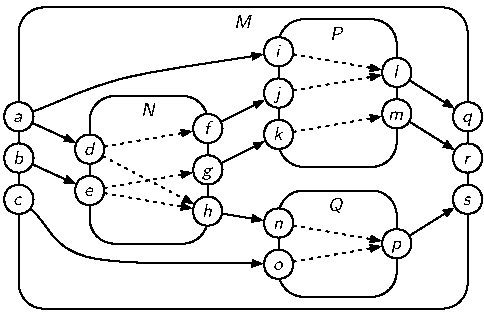
\includegraphics{compute-resume-state}
		\caption{Parent module with three submodules\label{fig:compute-resume-state-orig}}
	\end{subfigure}
	\quad
	\begin{subfigure}{8.2cm}
		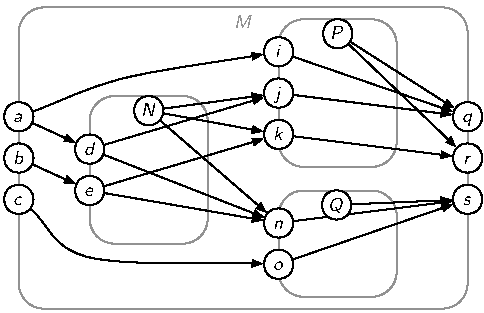
\includegraphics{compute-resume-state-dg}
		\caption{Corresponding dependency graph\label{fig:compute-resume-state-dg}}
	\end{subfigure}
	\caption{Example parent module and its dependency graph\label{fig:compute-resume-state}}
\end{figure}

\begin{example} \label{ex:module}
	Let $M = (I, O, L, \deps, S, C)$ be the CloudKeeper parent module shown in Figure~\ref{fig:compute-resume-state-orig}. The following list illustrates the previous definitions:
	\begin{itemize}
		\item Set of in-ports $I = \{ a, b, c \}$, set of out-ports $O = \{ q, r, s \}$, set of in-port/out-port pairs $L = \emptyset$
		\item Since $M$ is a parent module, function $\deps$ could be computed from the other elements in $M$. There is some freedom here: Strictly speaking, computing a value for out-port $q$ requires only a value for in-port $a$. That is, $q \in \deps(a)$ needs to hold necessarily, but it is optional that $q \in \deps(b)$ or $q \in \deps(c)$. We will see later that keeping sets $\deps$ minmal is most efficient, but it requires more preprocessing.

		The dashed lines indicate functions $\deps_N$, $\deps_P$ and $\deps_Q$. For instance, $\deps_N(d) = \{ f, h \}$, $\deps_N(e) = \{ g, h \}$, $\deps_P(i) = \{ l \}$, etc.
		\item Set of submodules $S = \{ N, P, Q \}$
		\item Set of parent-in-to-child-in connections $\Cparentchild = \{ (a, i), (a, d), (b, e), (c, o) \}$
		\item Set of sibling connections $\Csibling = \{ (f, j), (g, k), (h, n) \}$
		\item Set of child-out-to-parent-out connections $\Cchildparent = \{ (l, q), (m, r) \}, (p, s) \}$
		\item Set of short-circuit connections $\Cshort = \emptyset$
	\end{itemize}
	The corresponding dependency graph is shown in Figure~\ref{fig:compute-resume-state-dg}. Witnesses between dependency-graph vertices are, e.g., $\outports(a, i) = \emptyset$, $\outports(d, j) = \{ f \}$, $\outports(N, j) = \{ f \}$.
\end{example}

\subsection{The Basic Interpreter Protocol}

The CloudKeeper interpreter component provides module interpreters for the different kinds of modules, such as composite, loop, or simple modules. Despite idiosyncrasies that will be explained in this and later sections, all module interpreters adhere to the same basic protocol: In particular, module interpreters are always invoked asynchronously, and they communicate with the entity invoking them through a very simple message interface. Specifically, a module-interpreter invocation:
%
\begin{itemize}
	\item Receives \emph{in-port-has-value} messages from its invoker whenever one of its in-ports receives a value.
	\item Sends \emph{out-port-has-value} messages to its invoker whenever it has computed the value of an out-port.
	\item Receives a message during initialization that consists of two sets $I^*$ and $O^*$, where $I^*$ contains the in-ports for which in-port-has-value messages will be received, and $O^*$ contains the out-ports for that out-port-has-value messages have to be sent.
\end{itemize}
%
Whenever unambiguous or irrelevant, we will simply write module interpreter instead of module-interpreter invocation in the following.

CloudKeeper module interpreters do not differentiate between starting and resuming. Instead, when a module interpretation is started, it is always assumed that ports may have previously computed values. For efficiency, as many as possible of these values should be reused. Yet, not all values \emph{can} always be salvaged, because consistency requires that recomputing the value of a port also triggers reevaluation of all downstream ports.


\subsection{Parent-Module Interpreters} \label{sec:parentinterpreter}

The central piece of the interpreter component is the parent-module interpreter. It traverses a single parent module, such as a composite or a loop module, and is responsible for recursively starting interpreters for its submodules.

\paragraph{Consistent Checkpoints}

When a parent-module interpreter starts, it uses the sets $I^*$ and $O^*$ to compute a set of vertices $A$ in the dependency graph that constitute a \emph{consistent checkpoint}. Only then the traversal of the module will be started/resumed from this checkpoint. Specifically, consistent checkpoints used by CloudKeeper are characterized by the following properties:
%
\begin{enumerate}
	\item \label{prop:checkpoint:a} Each vertex in $A$ either represents a port that has a value or it represents a submodule.
	\item \label{prop:checkpoint:b} Resuming interpretation from all vertices in $A$ and from all in-port vertices in $I^*$ (once they receive a value) eventually leads to the computation of all required out-ports $O^*$. Formally, every maximal path ending in $O^*$ contains a vertex from $A \cup I^*$.
	\item \label{prop:checkpoint:c} No port will receive a new value more than once. Formally, every path that ends in $O^*$ contains at most one vertex from $A \cup I^*$.
	\item \label{prop:checkpoint:d} The number of reused values is maximal under the given constraints. Formally, the set of all vertices reachable from any other set $B$ satisfying the previous constraints is a superset of the set of all vertices reachable from $A$.
\end{enumerate}
%
The following Definition~\ref{def:consistentcp} formalizes and summarizes properties~\eqref{prop:checkpoint:a}--\eqref{prop:checkpoint:c}. It will be established in the next Section~\ref{sec:computecp} that the algorithm used by CloudKeeper even computes \emph{optimal} consistent checkpoints in the sense of property~\eqref{prop:checkpoint:d}.

\begin{definition} \label{def:consistentcp}
	Let $M = (I, O, L, \deps, S, C)$ be a parent module, $I^* \subseteq I$ be the set of recomputed in-ports, $O^* \subseteq O$ be the set of requested out-ports, and let $G = (V,E)$ be the pruned dependency graph. Let $H \subseteq V \setminus S$ be the set of ports that already have a value. A \emph{consistent checkpoint} $A \subseteq H \cup S \setminus I^*$ is a set of vertices so that every maximal path ending in $O^*$ contains exactly one vertex from $A \cup I^*$.
\end{definition}

\paragraph{Starting module interpreters}

Once a consistent checkpoint $A$ has been computed, the parent-module interpreter proceeds as follows:
\begin{itemize}
	\item It transmits the values from all in-ports contained in $A$ to all connection targets from which $O^*$ is reachable,
	\item it invokes a child interpreter for every submodule that has an in-port contained in $A$,
	\item it invokes a child interpreter for every submodule contained in $A$ that does not have any in-ports, and
	\item it sends out-port-has-value messages to its invoker for all out-ports contained in $A$.
\end{itemize}
%
As discussed above, for each child-interpreter invocation the set of recomputed in-ports and the set of requested out-ports is needed. These two sets can be inferred from the consistent checkpoint $A$ and the pruned dependency graph $G = (V,E)$. When invoking a child interpreter for submodule $N \in S$:
\begin{itemize}
	\item The set of recomputed in-ports are those vertices in $I_N$ that are reachable from $A$ (as they will receive a value later), but not itself in $A$ (as those already have a value).
	\item The set of requested out-ports are those vertices in $O_N$ that are also in
        \begin{gather}
        	W := \bigcup_{\substack{(v,w) \in E\\v \text{ reachable from } A \cup I^*}} \outports(v, w)\SiM. \label{eq:W}
        \end{gather}
\end{itemize}

\paragraph{Finishing a parent-module interpretation}

After every transmission of a value, one of the following actions takes place:
\begin{itemize}
	\item When a submodule in-port receives a value, the child interpreter is invoked if it has not been invoked before. An in-port-has-value message is sent to the child interpreter.
	\item When an out-port receives a value, an out-port-has-value message is sent to the invoker of the current interpreter.
\end{itemize}

Whenever the parent-module interpreter receives an out-port-has-value message from one of its child interpreters, it transmits the value from that submodule's out-port to all connection targets from which $O^*$ is reachable. This asynchronous sequence of events continues until all requested out-ports have a value.

\subsection{Computing Consistent Checkpoints} \label{sec:computecp}

While the previous section gave a definition for (and used) consistent checkpoints, we still need to verify that the definition is sound -- that is, consistent checkpoints really exist -- and that they can be computed efficiently. Both aspects are addressed by Algorithm~\ref{alg:resume}. Its basic idea is to perform a modified breadth-first-search in order to classify all vertices of the dependency graph into one of three categories:
%
\begin{description}
	\item[Ready] These vertices are exactly those contained in the consistent checkpoint. That is, these vertices do not need further input, and interpretation can resume immediately from these vertices. It is guaranteed that they will never receive a new value while the current module is interpreted.
	\item[Recompute] These are the vertices that are reachable from $I^*$ or a ``Ready'' vertex. They are guaranteed to receive a new value while the current module is interpreted.
	\item[Irrelevant] These are all other vertices, which are not needed during the current module interpretation. It is guaranteed that they will not receive a new value while the current module is interpreted.
\end{description}
%
The algorithm also computes the set $W$ from \eqref{eq:W}, which contains all submodules' out-ports that witness connections between $\ready$ or $\recompute$ vertices to another vertex with state $\recompute$. As stated previously, these are needed for recursive invocations of submodule interpreters.

\paragraph{The Formal Algorithm}

Apart from the inputs mentioned before, Algorithm~\ref{alg:resume} also takes as input the \emph{kind} of queue to be used; that is, a data structure with the following operations:
\begin{description}
	\item[enqueue$(x)$] Adds an element $x$ to the queue.
	\item[dequeue] Returns an element $x$ from the queue, provided that dequeue has returned $x$ fewer times than enqueue$(x)$ has been called.
	\item[isEmpty] Returns whether the queue is empty.
	\item[contains$(x)$] Returns whether $x$ is contained in the queue. This must be \emph{true} if after the last enqueue$(x)$, no dequeue operation has returned $x$. And this must return \emph{false} if dequeue has returned $x$ at least as often as enqueue$(x)$ has been called. Given a queue $Q$, we will use the shorthand notation ``$x \in Q$''.
\end{description}
%
Note that this specification can be met by different kinds of queues: For instance, one kind of queue may contain the same element more than once, while another could employ set semantics. Likewise, the order in which elements are dequeued could just be the insertion order, or it could be determined by (implicit) element priorities.

\begin{algorithm}[ComputeResumeState$(M, H, I^*, O^*)$] \label{alg:resume}
\alginput{parent module $M = (I, O, L, \deps, S, C)$,\\
	set $H \subseteq V \setminus S$ of ports that already have a value,\\
	set $I^* \subseteq I$ of recomputed in-ports,\\
	non-empty set $O^* \subseteq O$ of requested out-ports,\\
	kind of queue}
\algoutput{map $\state: V \to \{ \irrelevant, \ready, \recompute \}$,\\
	set $W = \bigcup_{(v,w) \in E \mid \state[v] \neq \irrelevant} \outports(v, w) \subseteq R$}
\algprecond{for all $i \in I$ with $\deps(i) \cap O^* \neq \emptyset: i \in H \cup I^*$}
\begin{algorithmic}[1]
	\State Construct dependency graph $G = (V,E)$, pruned w.r.t.\ $O^*$ \label{alg:resume:init-start}
	\State $Q \set$ new instance of the given kind of queue \label{alg:resume:create-queue}
	\For{$v \in V \setminus (I^* \cup O^*)$}
		\State $\state[v] \set \irrelevant$
	\EndFor
	\For{$i \in I^*$}
		\State $\state[i] \set \recompute$ \label{alg:resume:state0}
		\State enqueue $i$ to $Q$ \label{alg:resume:enqueue0}
	\EndFor
	\For{$o \in O^*$}
		\State $\state[o] \set \ready$ \label{alg:resume:state1}
		\State enqueue $o$ to $Q$ \label{alg:resume:enqueue1}
	\EndFor
	\State $W \set \emptyset$ \label{alg:resume:init-end}
	\While{$Q$ not empty} \label{alg:resume:loop}
		\State $v \set$ dequeue from $Q$ \label{alg:resume:dequeue}
		\If{$\state[v] = \ready$ and $v \not\in H \cup S$ \label{alg:resume:if0}}
			\State $\state[v] \set \recompute$ \label{alg:resume:state4}
		\EndIf
		\If{$\state[v] = \recompute$}
			\For{$w \in V$ with $(w,v) \in E$}
				\If{$\state[w] = \irrelevant$}
					\State $\state[w] \set \ready$ \label{alg:resume:state2}
					\State enqueue $w$ to $Q$ \label{alg:resume:enqueue2}
				\EndIf
			\EndFor
		\EndIf
		\For{$w \in V$ with $(v,w) \in E$}
			\State $W \set W \cup \outports(v,w)$ \label{alg:resume:outports}
			\If{$\state[w] \neq \recompute$}
				\State $\state[w] \set \recompute$ \label{alg:resume:state3}
				\State enqueue $w$ to $Q$ \label{alg:resume:enqueue3}
			\EndIf
		\EndFor
	\EndWhile
\end{algorithmic}
\end{algorithm}

\begin{example}
	Figure~\ref{fig:compute-resume-state-result} shows the result of running Algorithm~\ref{alg:resume} on the module from Example~\ref{ex:module}. The set $H$ consists of all vertices with a gray background. The set $I^*$ of recomputed in-ports is $\{ a \}$, and the set $O^*$ of requested out-ports is $\{ r, s \}$. Note that the pruned dependency graph only contains edges that are on a path to one of the requested out-ports.

	The result is indicated as follows: If a vertex $v \in V$ is shown with a thick stroke, then $\state[v] = \ready$, if it is shown with a dashed outline, then $\state[v] = \recompute$, and otherwise $\state[v] = \irrelevant$.
\end{example}

\begin{figure}[htb]
	\centering
	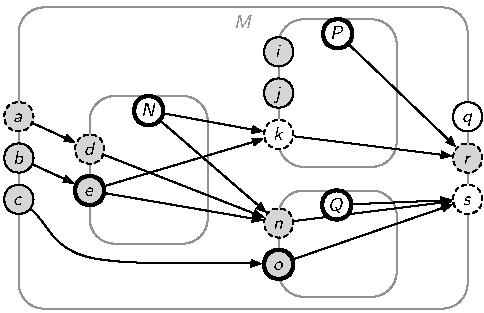
\includegraphics{compute-resume-state-result}
	\caption{Result of running Algorithm~\ref{alg:resume} \label{fig:compute-resume-state-result}}
\end{figure}

\paragraph{Termination and Runtime}

Computing the pruned dependency graph in line~\ref{alg:resume:init-start} can be done using, e.g., a breadth-first-search starting from the vertices in $O^*$. The initialization steps in lines~\ref{alg:resume:create-queue} to \ref{alg:resume:init-end} perform $|V|$ plus constantly many assignments and at most $|V|$ enqueuing operations. In the following, we verify termination and running time of the while-loop that starts in line~\ref{alg:resume:loop}. Every vertex $v \in V$ can be added to the queue only if $\state[v] = \ready$ (lines~\ref{alg:resume:enqueue1} and \ref{alg:resume:enqueue2}) or if $\state[v] = \recompute$ (lines \ref{alg:resume:enqueue0} and \ref{alg:resume:enqueue3}). Moreover, each enqueuing operation is contingent on $\state[v]$ having been modified in the immediately preceding line. Since the state of a vertex can only change from $\irrelevant$ to $\ready$ (lines~\ref{alg:resume:state1} and \ref{alg:resume:state2}) or from $\irrelevant$ or $\ready$ to $\recompute$ (lines \ref{alg:resume:state0} and \ref{alg:resume:state3}), this implies that every $v \in V$ can be enqueued at most twice -- in which case it would first be enqueued in state $\ready$ (line~\ref{alg:resume:enqueue1} or \ref{alg:resume:enqueue2}) and then again during some later iteration in state $\recompute$ (line~\ref{alg:resume:enqueue3}). Since one vertex is dequeued during every iteration of the while-loop (line~\ref{alg:resume:dequeue}), the queue will necessarily become empty during some iteration, at which point the algorithm will terminate. Specifically, the previous observation guarantees that there will be at most $2 |V|$ iterations of the while-loop.

\paragraph{Correctness}

We need to verify that, upon termination of Algorithm~\ref{alg:resume}, the set $A := \{ v \in V \mid \state[v] = \ready \}$ is a consistent checkpoint. This will proceed in a series of steps. First, we verify in Lemma~\ref{thm:resume:HuS} that $A$ contains no ``forbidden'' vertices. Then, we show in Lemmas~\ref{thm:resume:allpaths} and \ref{thm:resume:recomputenodes} and Corollary~\ref{thm:resume:exactlyone} that every maximal path ending in a required-out-port vertex contains exactly one vertex from $A$ or exactly one recomputed-in-port vertex, but not both.

We also need to verify that Algorithm~\ref{alg:resume} correctly computes set $W$ (containing all submodules' out-ports that must receive a new value). Lemma~\ref{thm:resume:W} establishes that $W$ is indeed as defined in \eqref{eq:W}.

\begin{lemma} \label{thm:resume:HuS}
	Upon termination of algorithm~\ref{alg:resume}, it holds for every $v \in V$ with $\state[v] = \ready$ that $v \in H \cup S \setminus I^*$.
\end{lemma}

\begin{proof}
	Let $v \in V$ with $\state[v] = \ready$. Setting $\state[v]$ to $\ready$ can only have happened in lines~\ref{alg:resume:state1} or \ref{alg:resume:state2}. In either case, $v$ was enqueued to $Q$ in the immediately succeeding line. Since the algorithm terminated, $v$ must have been dequeued in line~\ref{alg:resume:dequeue} in some subsequent iteration $i$ of the while-loop. The if-condition in the following line~\ref{alg:resume:if0} was not satisfied, because otherwise $\state[v]$ would have been updated to $\recompute$ (and would have remained $\recompute$ until the end of the algorithm). The first part of the if-condition, i.e., $\state[v] = \ready$, was satisfied in  iteration $i$, so it must have been the second part that was not satisfied. That is, $v \in H \cup S$. Moreover, $v \notin I^*$ because otherwise $\state[v]$ would have been set to $\recompute$ already in line~\ref{alg:resume:state0}.
\end{proof}

\begin{lemma} \label{thm:resume:allpaths}
	Let $(v_0, \dots, v_m)$ be a path in the dependency graph. Upon termination of Algorithm~\ref{alg:resume}, the following equivalence holds for every $j \in \{ 1, \dots, m \}$:
	\begin{gather*}
		\state[v_{j-1}] \neq \irrelevant \Longleftrightarrow \state[v_j] = \recompute\SiM.
	\end{gather*}
\end{lemma}

\begin{proof}
Let $n$ be the number of iterations of the while-loop before algorithm~\ref{alg:resume} terminates. Denote by $Q^{(0)}$ the set of vertices contained in queue $Q$ before entering the while-loop in line~\ref{alg:resume:loop}. Similarly, let $\state^{(0)}$ be the value of $\state$ at this point in the algorithm. For $i = 1, \dots, n$, denote by $Q^{(i)}$ and $\state^{(i)}$ the contents of $Q$ and $\state$, respectively, at the end of iteration $i$ of the while-loop. Obviously, $Q^{(0)} = I^* \cup O^*$ and $Q^{(n)} = \emptyset$.

We will show by induction over $i = 0, 1, \dots, n$ that the following invariant holds before and after each loop iteration.
\begin{quote}
	For every path $(v_0, \dots, v_m)$ in the dependency graph and every $j = 1, \dots, m$, the following implications hold:
	\begin{enumerate}
		\item \label{proof:resume:1} $\state^{(i)}[v_{j-1}] \neq \irrelevant$ and $\state^{(i)}[v_j] \neq \recompute \Longrightarrow v_{j-1} \in Q^{(i)}$
		\item \label{proof:resume:2} $\state^{(i)}[v_{j-1}] = \irrelevant$ and $\state^{(i)}[v_j] = \recompute  \Longrightarrow v_j \in Q^{(i)}$
	\end{enumerate}
\end{quote}
If this invariant holds after iteration~$n$, then this completes the proof because $Q^{(n)} = \emptyset$.

We first verify the base case $i = 0$. Let $(v_0, \dots, v_m)$ be a path and $j \in \{ 1, \dots, m\}$. To see~\eqref{proof:resume:1}, note that $\state^{(0)}[v_{j-1}] \neq \irrelevant$ implies $v_{j-1} \in I^* \cup O^*$. However, $v_{j-1}$ is not a sink vertex, so $v_{j-1} \notin O^*$, but instead $v_{j-1} \in I^*$. Due to line~\ref{alg:resume:enqueue0}, this implies $v_{j-1} \in Q^{(0)}$. Implication~\eqref{proof:resume:2} holds vacuously because the assumption is never satisfied: To see this, note that $\state^{(0)}[v_j] = \recompute$ implies $v_j \in I^*$, meaning that $v_j$ is a source vertex -- a contradiction.

Before continuing with the inductive step, we first need a small technical observation:
\begin{claim} \label{alg:resume:claim}
	Let $v \in V$, $i \in \{ 1, \dots, n \}$, $v \notin Q^{(i - 1)}$, and $v \notin Q^{(i)}$. Then $\state^{(i)}[v] = \state^{(i - 1)}[v]$.
\end{claim}
\begin{subproof}[of Claim~\ref{alg:resume:claim}]
	Since $v \notin Q^{(i-1)}$, it holds that $v$ was not dequeued from $Q$ in iteration~$i$, and therefore line~\ref{alg:resume:state4} cannot have modified $\state[v]$. Moreover, since $v$ was not enqueued to $Q$ in iteration~$i$, lines~\ref{alg:resume:state2} and \ref{alg:resume:state3} cannot have modified $\state[v_j]$, either. In order to see this, note that in each case the immediately following line would have enqueued $v$. Consequently, $\state^{(i)}[v] = \state^{(i - 1)}[v]$.
\end{subproof}

Now suppose that the invariant holds for an arbitrary iteration $i - 1 \in \{ 0, 1, \dots \}$. We show that the invariant also holds at the end of iteration $i$ (which proves the inductive step $i - 1 \to i$). Let $(v_0, \dots, v_m)$ be an arbitrary path, and let $j \in \{ 1, \dots, m\}$.

\begin{enumerate}
	\item By way of contradiction, assume that $v_{j-1} \notin Q^{(i)}$. If $v_{j-1} \in Q^{(i-1)}$, then $v_{j-1}$ was dequeued in iteration~$i$, and therefore $\state^{(i)}[v_j] = \recompute$ due to line~\ref{alg:resume:state3}, because $(v_{j-1}, v_j) \in E$. On the other hand, if $v_{j-1} \notin Q^{(i-1)}$, then at least one of the following holds because of the induction hypothesis (that is, because of the invariant after iteration $i - 1$):
	\begin{itemize}
		\item $\state^{(i-1)}[v_{j-1}] = \irrelevant$

		Since $v_{j-1} \notin Q^{(i)}$ and $v_{j-1} \notin Q^{(i-1)}$, Claim~\ref{alg:resume:claim} implies that also $\state^{(i)}[v_{j-1}] = \irrelevant$.

		\item $\state^{(i-1)}[v_j] = \recompute$

		In this case, also $\state^{(i)}[v_j] = \recompute$ because Algorithm~\ref{alg:resume} never changes the $\state$ of a vertex once it has been set to $\recompute$.
	\end{itemize}
	Hence, there is a contradiction to the assumption of implication~\eqref{proof:resume:1}, as needed.

	\item By way of contradiction, assume that $v_j \notin Q^{(i)}$. If $v_j \in Q^{(i-1)}$, then $v_j$ was dequeued in iteration~$i$. Therefore, either $\state^{(i)}[v_j] \neq \recompute$ or $\state[v_{j-1}]$ would have been set to $\ready$ in line~\ref{alg:resume:state2}, and thus $\state^{(i)}[v_{j-1}] \neq \irrelevant$, because $(v_{j-1}, v_j) \in E$. On the other hand, if $v_j \notin Q^{(i-1)}$, then at least one of the following holds because of the induction hypothesis:
	\begin{itemize}
		\item $\state^{(i-1)}[v_{j-1}] \neq \irrelevant$

		In this case, also $\state^{(i)}[v_{j-1}] \neq \irrelevant$ because Algorithm~\ref{alg:resume} never changes the $\state$ of a vertex back to $\irrelevant$.

		\item $\state^{(i-1)}[v_j] \neq \recompute$

		Since $v_j \notin Q^{(i)}$ and $v_j \notin Q^{(i-1)}$, Claim~\ref{alg:resume:claim} implies that also $\state^{(i)}[v_{j-1}] \neq \recompute$.
	\end{itemize}
	Hence, there is a contradiction to the assumption of implication~\eqref{proof:resume:2}, as needed.
\end{enumerate}
\end{proof}

\begin{lemma} \label{thm:resume:recomputenodes}
	Upon termination of Algorithm~\ref{alg:resume}, it holds for every $v \in V$ with $\state[v] = \recompute$ that $v$ is reachable from a vertex $w$ with $\state[w] = \ready$ or $w \in I^*$.
\end{lemma}

\begin{proof}
	Let $v \in V$ with $\state[v] = \recompute$, and let $v_0$ be a source vertex that $v$ is reachable from; that is, $v_0 \in I \cup S$. (Note that such a vertex $v_0$ always exists.) Since the ``reachable'' relation is transitive, it is sufficient to show the claim for $v_0$.

	If $\state[v_0] \neq \recompute$, then Lemma~\ref{thm:resume:allpaths}, together with a simple inductive argument, guarantees existence of a vertex $w$ with $\state[w] = \ready$ such that $v$ is reachable from $w$. Therefore suppose $\state[v_0] = \recompute$. One of the following must hold:
	\begin{itemize}
		\item $v_0 \in O^*$ (if $\state[v_0]$ was assigned in line~\ref{alg:resume:state0}),
		\item $v_0 \notin H \cup S$ (if assigned in line~\ref{alg:resume:state4}), or
		\item $\exists w \in V$ with $(w, v_0) \in E$ (if assigned in line~\ref{alg:resume:state3}).
	\end{itemize}
	Of these three cases, only $v_0 \notin H \cup S$ is compatible with the previous observation that $v_0 \in I \cup S$. By construction of the dependency graph, and since $\state[v_0] \neq \irrelevant$, some vertex in $O^*$ is reachable from $v_0$, implying $\deps(v_0) \cap O^* \neq \emptyset$. The precondition of Algorithm~\ref{alg:resume} implies that $v_0 \in H \cup I^*$. Put together, we get $v_0 \in I^*$.
\end{proof}

\begin{corollary} \label{thm:resume:exactlyone}
	Upon termination of Algorithm~\ref{alg:resume}, every maximal path ending in $O^*$ contains exactly one vertex $v$ with $\state[v] = \ready$ or $v \in I^*$.
\end{corollary}

\begin{proof}
	Let $(v_0, \dots, v_n)$ be a maximal path with $v_n \in O^*$. Existence of a $j \in \{ 0, \dots, n\} $ with $\state[v_j] = \ready$ or with $v_j \in I^*$ is established by Lemma~\ref{thm:resume:recomputenodes} and the fact that for all $o \in O^*$ it holds that $\state[o] \neq \irrelevant$.

	In order to show uniqueness, note that Lemma~\ref{thm:resume:allpaths} implies there is at most one $j \in \{ 0, \dots, n\} $ with $\state[v_j] = \ready$. In that case, $v_j \notin I^*$ because of Lemma~\ref{thm:resume:HuS}. By construction of the dependency graph, it moreover holds that $v_1, \dots, v_n \notin I^*$. This completes the proof.
\end{proof}

\begin{lemma} \label{thm:resume:W}
	Upon termination of Algorithm~\ref{alg:resume}, let $A := \{ v \in V \mid \state[v] = \ready\}$ be the computed checkpoint. It holds that
	\begin{gather*}
		W = \bigcup_{\substack{(v,w) \in E\\v \text{ reachable from } A \cup I^*}} \outports(v, w)\SiM.
	\end{gather*}
\end{lemma}

\begin{proof}
	Due to Lemmas~\ref{thm:resume:allpaths} and \ref{thm:resume:recomputenodes}, we know that a vertex $v \in V$ is reachable from $A \cup I^*$ if and only if $\state[v] \neq \irrelevant$.

	We first show ``$\subseteq$''. Let $o \in W$. Obviously, $o$ was added to $W$ in line~\ref{alg:resume:outports}, for some $v,w \in V$ with $o \in \outports(v,w)$. At the beginning of that while-loop iteration, $v$ was necessarily dequeued in line~\ref{alg:resume:dequeue}. This implies that $\state[v] \neq \irrelevant$ at that time. Since $\state[v]$ can never change back to $\irrelevant$, it also means that $\state[v] \neq \irrelevant$ after Algorithm~\ref{alg:resume} terminated.

	In order to show ``$\supseteq$'', let $(v, w) \in E$ with $\state[v] \neq \irrelevant$, meaning that $\state[v]$ was updated at least once either in line~\ref{alg:resume:state0}, \ref{alg:resume:state1}, \ref{alg:resume:state2}, or \ref{alg:resume:state3}. In each case, the subsequent line added $v$ to the queue. Since Algorithm~\ref{alg:resume} terminated, $v$ was dequeued later, implying that $\outports(v,w) \subseteq W$ due to line~\ref{alg:resume:outports}.
\end{proof}

\paragraph{Optimality}

So far, we have verified that Algorithm~\ref{alg:resume} correctly computes a consistent checkpoint $A$. In the following, we show that $A$ is moreover optimal in the following sense: If $B$ is any other consistent checkpoint, then the set of vertices reachable from $B$ is a superset of the set of vertices reachable from $A$.

\begin{lemma} \label{thm:resume:optimal}
	Let $B$ be a consistent checkpoint. Upon termination of algorithm~\ref{alg:resume}, it holds for all $v \in V$ with $\state[v] \neq \irrelevant$ that $v$ is reachable from $B \cup I^*$.
\end{lemma}

\begin{proof}
	Using the same notation as in the proof of Lemma~\ref{thm:resume:allpaths}, we show that the following invariant holds before and after every iteration of the while-loop. For every $v \in V$:
	\begin{quote}
		\begin{enumerate}
			\item \label{proof:mincp:1} $\state^{(i)}[v] \neq \irrelevant \Longrightarrow v$ reachable from $B \cup I^*$ and
			\item \label{proof:mincp:2} $\state^{(i)}[v] = \recompute \Longrightarrow v \notin B$.
		\end{enumerate}
	\end{quote}
	We first verify the base case $i = 0$ (that is, prove the invariant before the first iteration). Let $v \in V$. To see \eqref{proof:mincp:1}, note that $\state^{(0)}[v] \neq \irrelevant$ implies $v \in I^* \cup O^*$. Since $B$ is a consistent checkpoint, all vertices in $I^* \cup O^*$ must be reachable from $B \cup I^*$. To see \eqref{proof:mincp:2}, note that $\state^{(0)}[v] = \recompute$ implies $v \in I^*$. Again by definition of a consistent checkpoint, we know $I^* \cap B = \emptyset$.

	For the inductive step $i - 1 \to i$, it is sufficient to consider any arbitrary $w$ with $\state^{(i - 1)}[w] = \irrelevant$ and $\state^{(i)}[w] \neq \irrelevant$. Let $v$ be the vertex dequeued in line~\ref{alg:resume:dequeue} of iteration~$i$.

	There are two cases. If the assignment to $\state[w]$ happened in line~\ref{alg:resume:state2}, then $v$ is reachable from $B \cup I^*$ and $v \notin B$, both by the induction hypothesis. Moreover, $v \notin I^*$ because $v$ is not a source vertex. By way of contradiction, suppose now that $w$ is not reachable from $B \cup I^*$. Then we can find a maximal path containing $w$ and $v$ that does not contain a vertex from $B \cup I^*$; a contradiction to the assumption that $B$ is a consistent checkpoint. This proves \eqref{proof:mincp:1}. Since $\state^{(i)}[w] = \ready$, property \eqref{proof:mincp:2} holds vacuously.

	If the assignment happened in line~\ref{alg:resume:state3}, then likewise $w$ is reachable from $B \cup I^*$, because $(v,w) \in E$ and $v$ is reachable from $B \cup I^*$ by the induction hypothesis. To see \eqref{proof:mincp:2}, note that since $v$ is reachable from $B \cup I^*$, it must hold that $w \notin B$. Otherwise, there would be a path through $v$ and $w$ that contains more than one vertex from $B \cup I^*$. This completes the proof.
\end{proof}

\paragraph{Implementation}

Set $H$ is the set of all ports that already have a value. In practice, this set is relatively expensive to compute because doing so may involve accessing secondary storage (like the file system). It is therefore desirable to use $H$ only lazily, in particular because the only operation needed is ``$\notin$'' in line~\ref{alg:resume:if0}. It is additionally desirable to allow processing more than one such operation at a single time. Hence, the operation should not block, and the question is instead if one may asynchronously check $v \in H$ and not dequeue $v$ while the result is unknown. This would be possible if the order of dequeuing in line~\ref{alg:resume:dequeue} was arbitrary, and we can simply dequeue another vertex $w \neq v$ while waiting for $v$. The following Lemma~\ref{thm:resume:orderindependence} shows this is indeed the case.

\begin{lemma} \label{thm:resume:orderindependence}
	The output of Algorithm~\ref{alg:resume} does not depend on the kind of queue used.
\end{lemma}

\begin{proof}
	Let $M, H, I^*, O^*$ be arbitrary valid arguments for Algorithm~\ref{alg:resume}. Define $\state(\phi)$ as the output of Algorithm~\ref{alg:resume} with the previous arguments and using a queue of kind $\phi$. Let $A(\phi) := \{ v \in V \mid \state(\phi)[v] = \ready\}$ and let $X(\phi) := \{ v \in V \mid v \text{ reachable from } A(\phi) \cup I^*\}$.

	Lemma~\ref{thm:resume:optimal} shows that for any two $\phi, \phi'$, it holds that $X(\phi) \subseteq X(\phi')$. Consequently, $X(\phi)$ is constant in $\phi$. Let $Y$ denote this constant. We will show that not just $X(\phi)$ is constant in $\phi$, but also $\state(\phi)$ is constant in $\phi$. To this end, define $\state'$ as follows:
	\begin{gather*}
		\state'[v] := \begin{cases}
				\recompute & \text{if $v \in I^*$ or there is $w \in Y$ with $(w,v) \in E$} \\
				\ready & \text{if $v \in Y$ otherwise} \\
				\irrelevant & \text{otherwise}\SiM.
			\end{cases}
	\end{gather*}
	%
	Now let $\phi$ be an arbitrary kind of queue. We will show that $\state(\phi) = \state'$. Let $v \in V$; there are three cases:
	\begin{itemize}
		\item Suppose $\state'[v] = \recompute$. It holds that $v \in I^*$ or there is a $w \in V$ with $w$ reachable from $A(\phi) \cup I^*$ and $(w,v) \in E$. By Lemma~\ref{thm:resume:allpaths}, this implies $\state(\phi)[v] = \recompute$.
		\item Suppose $\state'[v] = \ready$. By definition of $\state'$, it holds that $v \notin I^*$ and that there is no $w \in X$ with $(w,v) \in E$. That is, there is no $w \in V$ with $(w,v) \in E$ such that $w$ is reachable from $A(\phi) \cup I^*$. However, $v \in Y = X(\phi)$, i.e., $v$ is reachable from $A(\phi) \cup I^*$. This implies $v \in A(\phi) \cup I^*$. Put together, $v \in A(\phi)$, which is equivalent to $\state'[v] = \ready$.
		\item Suppose $\state'[v] = \irrelevant$. In this case, $v \notin Y$, i.e., $v$ is not reachable from $A(\phi) \cup I^*$. By definition, $v \notin A(\phi)$ implies $\state(\phi)[v] \neq \ready$. Moreover, it follows from Lemma~\ref{thm:resume:recomputenodes} that $\state(\phi)[v] \neq \irrelevant$. Hence, $\state(\phi)[v] = \irrelevant$.
	\end{itemize}
	Since $\state(\phi) = \state'$, and due to Lemma~\ref{thm:resume:W}, the set $W$ computed by Algorithm~\ref{alg:resume} is likewise independent of $\phi$. This completes the proof.
\end{proof}

\end{document}
